\shorttitle{Двомасштабне стохастичне моделювання з агрегованим міжспільнотним зв'язком}
\shortauthors{Y. Kuryliak and M.T.M. Emmerich}

\title[mode=title]{Двомасштабне стохастичне моделювання епідемій у мережах спільнот: формулювання та точність агрегованого міжспільнотного зв'язку}

\author[1]{Yulian Kuryliak}[orcid=0000-0002-6600-2637]
\cormark[1]
\ead{yulian.a.kuryliak@lpnu.ua}
\affiliation[1]{organization={Інститут комп'ютерних наук та інформаційних технологій, Національний університет ``Львівська політехніка''},
            addressline={вул. Степана Бандери, 12},
            city={Львів},
            postcode={79000},
            country={Україна}}

\author[2]{Michael T. M. Emmerich}[orcid=0000-0002-7342-2090]
\ead{michael.t.m.emmerich@jyu.fi}
\affiliation[2]{organization={Факультет інформаційних технологій, Університет Ювяскюля},
            addressline={P.O. Box 35 (Agora)},
            city={Ювяскюля},
            postcode={FI-40014},
            country={Фінляндія}}

\cortext[1]{Автор для листування}

\begin{abstract}
У моделюванні епідемій у структурованих популяціях докладні мережі контактів усередині спільнот часто поєднують лише з агрегованою інформацією про контакти між ними. Ми досліджуємо двомасштабний стохастичний симулятор для таких умов, раніше стисло описаний у матеріалах семінару: кожна спільнота точно моделюється власним рушієм Gillespie, тоді як моменти міжспільнотних заражень визначаються агрегованими залежними від стану інтенсивностями, а зараження рівномірно розміщуються серед сприйнятливих вузлів спільноти-одержувача. Ми надаємо повну специфікацію методу, зокрема його сіткову синхронізацію, і показуємо, що його ідеальна версія є точним моделюванням сурогатної мережі, у якій кожен пучок міжспільнотних ребер замінено рівномірним зв'язком «усі з усіма» з такою самою сумарною вагою. Таке подання виявляє чотири джерела розбіжностей (втрата інформації про стан граничних вузлів, рівномірне розміщення, відсутність вичерпання ребер інтерфейсу та похибка синхронізації) й означає, що для випадково розміщених інтерфейсів ідеальний агрегований годинник експорту стохастично випереджає повномережевий. Ми порівняли метод із повномережевим моделюванням Gillespie динаміки SI у тестах з одиничним експортом і в 48 конфігураціях ланцюгів із десяти спільнот (50--1000 вузлів у спільноті, довжини внутрішніх шляхів 1--6, одне або п'ять ребер інтерфейсу, по 400 узгоджених запусків). Коли розкид часів зараження всередині спільноти був меншим за чверть середнього часу переходу через одне ребро, розподіли часу прибуття до кінцевої спільноти були статистично нерозрізненними у 15 із 18 конфігурацій; за більших значень двомасштабний симулятор прибував раніше на величину, приблизно пропорційну цьому відношенню, яка сягала 40\%. Близькість часів не означала допустимості маршрутів: до 52\% агрегованих переходів передували зараженню будь-якого справжнього вузла-моста.
\end{abstract}

\begin{highlights}
\item Точні локальні рушії Gillespie зв'язані через агреговані міжспільнотні інтенсивності
\item Ідеальна схема точно моделює сурогатну мережу з інтерфейсом «усі з усіма»
\item Для випадково розміщених інтерфейсів агреговані годинники експорту стохастично випереджають повномережеві
\item Точність визначається співвідношенням внутрішнього розкиду часів і часу переходу через ребро
\item Близькі часи прибуття можуть співіснувати з фізично неможливими маршрутами передавання
\end{highlights}

\begin{keywords}
Стохастичне моделювання \sep Алгоритм Gillespie \sep Багатомасштабне моделювання \sep Мережі спільнот \sep Моделювання епідемій \sep Похибка апроксимації
\end{keywords}

\maketitle

%======================================================================
\section{Вступ}
\label{sec:introduction}

Контактна структура популяції визначає поширення інфекції: неоднорідні та кластеризовані контакти змінюють епідемічні пороги, темпи зростання і часи прибуття порівняно з однорідним перемішуванням \citep{keeling2005,pastorsatorras2015,kiss2017}. У більших масштабах передавання між містами або регіонами зумовлене мобільністю, яку зазвичай описують потоками між місцевостями, а не індивідуальними контактами \citep{balcan2009,barbosa2018human}. Тому моделі таких систем мають справу з інформацією двох рівнів деталізації. Усередині спільноти мережу контактів можна спостерігати, реконструювати або синтезувати \citep{eubank2004,danon2011}. Між спільнотами часто доступні лише агреговані величини, як-от обсяги маятникової міграції або показники мобільності \citep{barbosa2018human,chang2021}.

Якби повна мережа контактів була відома, епідемія була б марковським ланцюгом із неперервним часом (CTMC), траєкторії якого можна точно генерувати алгоритмами типу Gillespie \citep{gillespie1977exact,gibson2000}; ефективні мережеві реалізації роблять це здійсненним для великих графів \citep{vestergaard2015,kuryliak2025simulating}. Проте точне моделювання вимагає задати кожен канал передавання, зокрема кожен контакт між спільнотами. Метапопуляційні моделі застосовують протилежний підхід: вони оперують агрегованими потоками, але водночас замінюють внутрішньоспільнотну динаміку компартментами \citep{colizza2007reaction,colizza2008,balcan2010modeling,ajelli2010}. Між цими крайнощами лежить практично важлива проміжна модель, у якій докладна стохастична мережева динаміка зберігається всередині спільнот, а агрегується лише інтерфейс між ними.

Двомасштабний симулятор такого типу було стисло описано в матеріалах семінару \citep{kuryliak2025towards}. Кожна спільнота моделюється власним точним рушієм Gillespie; макрорівень генерує міжспільнотні зараження на основі агрегованих інтенсивностей, що залежать від поточних часток інфікованих і сприйнятливих у спільнотах, а кожне імпортоване зараження розміщується у спільноті-одержувачі. У матеріалах семінару архітектуру обґрунтовано витратами на подання кожного міжспільнотного контакту та окреслено її рівні; аналіз похибки, внесеної агрегуванням, залишено наступним кроком. Оскільки той опис був стислим, тут ми подаємо метод у самодостатній формі.

Центральне питання цієї статті полягає в тому, наскільки точно агрегований інтерфейс відтворює повномережевий CTMC, який він замінює, для яких спостережуваних величин і в яких мережевих режимах. Відповідь залежить від інформації, яку відкидає інтерфейс: які саме вузли утворюють інтерфейс, куди потрапляє імпортоване зараження і скільки разів можна перетнути вузький інтерфейс. Ми досліджуємо це аналітично та за допомогою контрольованих обчислювальних експериментів, у яких повна мережа відома експериментатору, але двомасштабному симулятору передається лише її агреговане подання.

Основні внески цієї роботи такі.
\begin{enumerate}
\item Повна специфікація двомасштабного методу на рівні реалізації, зокрема застосованого на практиці сітково синхронізованого планувальника на основі інтеграла інтенсивності (Розділ~\ref{sec:method}, Алгоритм~\ref{alg:scheduler}).
\item Точна характеристика ідеального методу як повномережевого моделювання на сурогатній мережі з рівномірним міжспільнотним зв'язком «усі з усіма» (Твердження~\ref{prop:surrogate}). Вона дає таксономію розбіжностей і результат щодо стохастичного впорядкування одиничних експортів (Твердження~\ref{prop:ordering}).
\item Контрольоване порівняння з повномережевим моделюванням Gillespie у тестах з одиничним експортом і на ланцюгах спільнот із використанням перестановочних базових рівнів, що відокремлюють похибку апроксимації від вибіркової мінливості (Розділи~\ref{sec:design} і~\ref{sec:results}).
\item Практичний критерій: відношення розкиду часів зараження всередині спільноти до часу переходу через одне ребро впорядковує спостережувані розбіжності для різних розмірів спільнот, внутрішніх структур і ширин інтерфейсу (Розділ~\ref{sec:res_descriptor}).
\end{enumerate}

Дослідження обмежене динамікою «сприйнятливий--інфікований» (SI) на статичних синтетичних мережах і фіксованим кроком синхронізації. У Розділі~\ref{sec:related} метод зіставлено з наявними підходами до моделювання; у Розділі~\ref{sec:method} його специфіковано; у Розділі~\ref{sec:analysis} проаналізовано, що зберігає агрегований інтерфейс; у Розділах~\ref{sec:design} і~\ref{sec:results} описано експерименти та їхні результати; у Розділі~\ref{sec:discussion} обговорено практичне застосування, обчислювальні витрати й обмеження.

%======================================================================
\section{Пов'язані праці}
\label{sec:related}

\paragraph{Точне та наближене стохастичне моделювання.}
Прямий метод Gillespie точно генерує траєкторії CTMC за поточними схильностями реакцій \citep{gillespie1977exact}; метод наступної реакції організовує ті самі обчислення навколо окремих годинників каналів \citep{gibson2000}. Коли схильності змінюються з часом, точне моделювання можна виразити через подання процесу підрахунку випадковою заміною часу \citep{ethier1986}: подія відбувається, коли її інтегрована інтенсивність досягає незалежного експоненційного порога. \citet{anderson2007} перетворив це подання на модифікований метод наступної реакції для залежних від часу схильностей. Макрогодинник двомасштабного симулятора є прикладом такої конструкції зі стохастичною, залежною від стану інтенсивністю. Орієнтовані на мережі реалізації оновлюють лише схильності, на які вплинула подія \citep{vestergaard2015,kuryliak2025simulating}; використані тут локальні рушії відповідають \citet{kuryliak2025simulating}.

Гібридні та багатомасштабні алгоритми стохастичного моделювання пришвидшують системи з істотно розділеними швидкостями реакцій, наближено відтворюючи швидкі канали \citep{haseltine2002,cao2005slow}. Двомасштабний метод відрізняється об'єктом апроксимації: він не усереднює швидкі канали, а вилучає інформацію про те, які міжспільнотні канали активні. Проте, як показано в Розділі~\ref{sec:results}, його точність також упорядковується розділенням часових масштабів, а саме між внутрішнім поширенням і переходом через інтерфейс.

\paragraph{Метапопуляційні моделі та моделі мобільності.}
Метапопуляційні моделі зв'язують субпопуляції потоками мобільності; їх застосовували для дослідження порогів вторгнення та глобального поширення \citep{colizza2007reaction,colizza2008,balcan2009,balcan2010modeling}; мережі мобільності високої роздільної здатності можна поєднувати з локальними моделями передавання \citep{chang2021}. Агентні моделі описують окремих індивідів у всій системі \citep{eubank2004,kerr2021}, а \citet{ajelli2010} порівняв ці дві парадигми. Двомасштабний метод зберігає окремі вузли та контакти всередині спільнот, а отже, локальну стохастичність і мережеву структуру, проте між спільнотами використовує лише інформацію метапопуляційного типу.

\paragraph{Два рівні перемішування та спільне моделювання.}
Епідемічні моделі з двома рівнями перемішування поєднують локальні контакти в малих групах із рівномірним глобальним перемішуванням \citep{ball1997}. Сурогатна мережа з Твердження~\ref{prop:surrogate} має таку саму структуру, де глобальне перемішування обмежене парами спільнот і зважене агрегованим зв'язком. З погляду програмної організації моделювання двомасштабний планувальник є головним компонентом спільного моделювання, який просуває підсистеми як «чорні скриньки» по комунікаційній сітці й обмінюється невеликою кількістю змінних зв'язку \citep{gomes2018cosim}. На відміну від типових інтерфейсів спільного моделювання, тут інтерфейс не лише передає стан, а й визначає, коли і де у підсистемі-одержувачі відбуваються стохастичні події.

%======================================================================
\section{Метод двомасштабного моделювання}
\label{sec:method}

\subsection{Повномережева еталонна модель}
\label{sec:reference}

Нехай $G=(V,E)$ --- мережа контактів, множину вузлів якої розбито на $M$ спільнот, $V=\bigsqcup_{i=1}^{M}V_i$, де $N_i=|V_i|$. Ми розглядаємо $E$ як множину орієнтованих каналів передавання; неорієнтований контакт утворює два канали. Канали поділено на внутрішньоспільнотні пучки $E_{ii}$ і міжспільнотні пучки $E_{ij}=\{(u,v)\in E:u\in V_i,\,v\in V_j\}$, $i\neq j$. Кожен вузол є сприйнятливим ($S$), інфікованим ($I$) або видаленим ($R$). Для конфігурації $x\in\{S,I,R\}^V$ позначимо через $x^{v:I}$ і $x^{u:R}$ конфігурації, у яких вузол $v$ став інфікованим або вузол $u$ був видалений відповідно. Повномережевий процес є CTMC з генератором
\begin{equation}
\label{eq:full_generator}
(\mathcal{L}_G f)(x)=\sum_{(u,v)\in E}\beta_{uv}\,\ind\{x_u=I,\,x_v=S\}\bigl[f(x^{v:I})-f(x)\bigr]
+\sum_{u\in V}\gamma\,\ind\{x_u=I\}\bigl[f(x^{u:R})-f(x)\bigr],
\end{equation}
де $\beta_{uv}$ --- інтенсивність передавання каналу $(u,v)$, а $\gamma$ --- інтенсивність видалення. Міжспільнотні інтенсивності записуємо як $\beta_{uv}=\beta_{\mathrm{out}}w_{uv}$, де $w_{uv}$ --- ваги контактів. Точне моделювання~\eqref{eq:full_generator} ми називаємо \Full{}. В усіх експериментах цієї статті використано динаміку SI ($\gamma=0$).

\subsection{Агрегований інтерфейс}
\label{sec:interface}

Двомасштабний симулятор, позначений \TS{}, отримує внутрішньоспільнотні графи $G_i=(V_i,E_{ii})$ з їхніми інтенсивностями, але не міжспільнотні пучки. Кожен пучок подано лише його агрегованою вагою
\begin{equation}
\label{eq:weight}
W_{ij}=\sum_{(u,v)\in E_{ij}}w_{uv},\qquad i\neq j,
\end{equation}
яка для одиничних ваг дорівнює кількості каналів із $V_i$ до $V_j$. У прикладних задачах $W_{ij}$ оцінювали б за даними досліджень мобільності або контактів, а не обчислювали з відомої мережі. Стан спільноти $i$ узагальнюється кількостями $s_i$ і $y_i$ сприйнятливих та інфікованих вузлів і відповідними частками $\sbar_i=s_i/N_i$ та $\ibar_i=y_i/N_i$. У Таблиці~\ref{tab:information} наведено інформацію, яку використовує кожна модель. На Рисунку~\ref{fig:schematic}(a,b) зіставлено два подання.

\begin{table}[tbp]
\centering
\caption{Інформація, яку використовують повномережева еталонна модель і двомасштабний симулятор.}
\label{tab:information}
\small
\begin{tabular}{>{\raggedright\arraybackslash}p{0.38\linewidth}>{\raggedright\arraybackslash}p{0.25\linewidth}>{\raggedright\arraybackslash}p{0.27\linewidth}}
\toprule
Елемент & \Full{} & \TS{}\\
\midrule
Внутрішньоспільнотні контакти та інтенсивності & так & так\\
Стани вузлів усередині спільнот & так & так (локальні рушії)\\
Міжспільнотні канали $E_{ij}$ (вузли-мости та кінцеві вузли) & так & ні\\
Агрегована вага $W_{ij}$ & випливає з $E_{ij}$ & так\\
Інтенсивність передавання з $V_i$ до $V_j$ & зі станів каналів у $E_{ij}$ & з $\ibar_i$, $\sbar_j$ і $W_{ij}$\\
Вузол-одержувач передавання & кінцевий вузол каналу, що спрацював & вибирається за правилом розміщення\\
Максимальна кількість передавань через пучок (SI) & кількість каналів & обмежена лише $s_j$\\
\bottomrule
\end{tabular}
\end{table}

\begin{figure}[tbp]
\centering
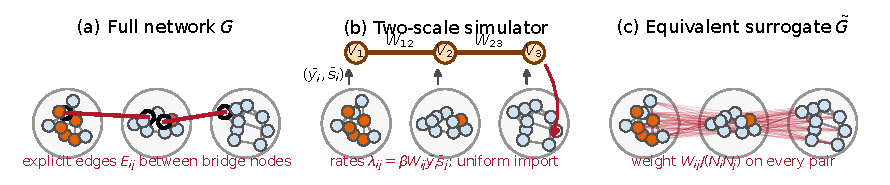
\includegraphics[width=\linewidth]{Images/twoscale/fig_method_schematic.pdf}
\caption{(a) Повна мережа: інфекція переходить між спільнотами лише явними ребрами, що з'єднують вузли-мости (чорні кільця). (b) Двомасштабний симулятор: кожна спільнота є точним локальним рушієм Gillespie; макрорівень бачить лише частки $(\ibar_i,\sbar_i)$ й агреговані ваги $W_{ij}$, генерує міжспільнотні зараження з інтенсивностями $\lambda_{ij}$ і розміщує кожен імпорт на рівномірно вибраному сприйнятливому вузлі. (c) Еквівалентна сурогатна мережа з Твердження~\ref{prop:surrogate}: кожна пара вузлів у сусідніх спільнотах з'єднана слабким ребром ваги $W_{ij}/(N_iN_j)$. Помаранчеві вузли --- інфіковані; сині --- сприйнятливі.}
\label{fig:schematic}
\end{figure}

\subsection{Локальні рушії}
\label{sec:local}

Кожна спільнота моделюється окремим рушієм, який генерує траєкторії CTMC її власного графа $G_i$: зараження вздовж каналів у $E_{ii}$ та видалення інфікованих вузлів зі схильностями з~\eqref{eq:full_generator}, обмеженими на $V_i$. Рушії використовують інкрементну реалізацію Gillespie з \citet{kuryliak2025simulating}, у якій кожен вузол зберігає сумарну вагу своїх контактів з інфікованими сусідами, а оновлюються лише схильності, на які вплинула подія. Кожен рушій має власний незалежний потік псевдовипадкових чисел.

Рушій підтримує дві операції, які використовує макрорівень: просування його годинника до заданого моменту із застосуванням лише тих подій, що відбуваються раніше за нього, та \emph{імпорт}, який переводить заданий сприйнятливий вузол у стан $I$. Імпорт змінює локальні схильності; тому рушій відкидає наступну заплановану подію і генерує нову з оновленого стану. Оскільки часи очікування CTMC не мають пам'яті, такий перезапуск зберігає закон локального процесу. Між імпортами кожен рушій є точним моделюванням своєї ізольованої спільноти.

\subsection{Макрорівень}
\label{sec:macro}

Макрорівень розглядає спільноти як вузли зваженого графа з вагами $W_{ij}$. За поточними узагальненнями стану він призначає кожній упорядкованій парі $i\neq j$ інтенсивність
\begin{equation}
\label{eq:macro_rate}
\lambda_{ij}(t)=\beta_{\mathrm{out}}\,W_{ij}\,\ibar_i(t)\,\sbar_j(t),
\qquad
\Theta(t)=\sum_{i\neq j}\lambda_{ij}(t).
\end{equation}
Макроподія --- це одиничне зараження, передане з однієї спільноти до іншої. Коли вона відбувається, пару $(i,j)$ вибирають з імовірністю $\lambda_{ij}/\Theta$, а цільовий вузол $v\in S_j$ --- за правилом розміщення $\Pi_{ij}(\cdot\mid x)$. Стандартне правило, використане в усій статті, є рівномірним розміщенням, $\Pi_{ij}(v\mid x)=1/s_j$. Якщо така інформація доступна, можна застосовувати правила, зважені за степенем вузла або з урахуванням межі. Реалізація також містить мультиплікативний калібрувальний коефіцієнт для~\eqref{eq:macro_rate}, який було встановлено рівним одиниці.

За заданих кількостей вузлів у станах спільнот інтенсивність~\eqref{eq:macro_rate} є математичним сподіванням інтенсивності пучка $E_{ij}$, коли його кінцеві вузли розміщені рівномірно випадково. Вона збігається з фактичною інтенсивністю, коли пучок з'єднує кожну пару вузлів однаковою вагою (Наслідок~\ref{cor:exact}), і є наближенням в інших випадках (Розділ~\ref{sec:analysis}). Макрорівень не є автономним: $\Theta$ змінюється щоразу, коли локальна подія або імпорт змінює кількість вузлів у станах певної спільноти. Оскільки між такими подіями узагальнення стану є кусково сталими, $\Theta$ також кусково стала.

\subsection{Час за інтегралом інтенсивності та синхронізація}
\label{sec:timing}

Нехай $t_0$ --- час попередньої макроподії, а $E\sim\Exp(1)$ --- незалежний поріг. В ідеальній конструкції наступна макроподія відбувається в момент
\begin{equation}
\label{eq:hazard_integral}
t^\ast=\inf\Bigl\{t>t_0:\int_{t_0}^{t}\Theta(s)\,ds\ge E\Bigr\},
\end{equation}
що є поданням процесу підрахунку з інтенсивністю $\Theta$ через випадкову заміну часу \citep{ethier1986,anderson2007}. Для сталої $\Theta$ воно зводиться до часу очікування Gillespie $(t^\ast-t_0)=-\ln U/\Theta$, $U\sim\mathcal{U}(0,1)$. У поєднанні з точними локальними рушіями конструкція~\eqref{eq:hazard_integral} визначає \emph{ідеальний} двомасштабний процес, інтенсивності переходів якого наведено в Розділі~\ref{sec:surrogate}.

Реалізований планувальник (Алгоритм~\ref{alg:scheduler}) трактує локальні рушії як «чорні скриньки», що відкривають свій стан лише після просування. Він ділить час на інтервали синхронізації довжини $\tau$ й оцінює $\Theta$ на кожному (під)інтервалі $[t,t_g)$ за пробою в середній точці: копії всіх рушіїв, разом зі станами їхніх генераторів випадкових чисел, просуваються до $t+\Delta/2$, де $\Delta=t_g-t$, після чого за копіями обчислюється $\Theta_{\mathrm{mid}}$. Якщо накопичена інтенсивність $A+\Theta_{\mathrm{mid}}\Delta$ залишається нижчою за $E$, фактичні рушії просуваються до $t_g$. Інакше момент перетину інтерполюється як
\begin{equation}
\label{eq:interpolation}
t^\ast=t+\frac{E-A}{\Theta_{\mathrm{mid}}},
\end{equation}
рушії просуваються до $t^\ast$, а пару та цільовий вузол вибирають за їхніми станами в момент $t^\ast$. Потім поріг поновлюється, й у такий самий спосіб обробляється решта інтервалу.

\begin{algorithm}[tbp]
\caption{Сітково синхронізоване двомасштабне моделювання однієї реалізації.}
\label{alg:scheduler}
\small
\begin{tabbing}
\hspace*{1.6em}\=\hspace*{1.4em}\=\hspace*{1.4em}\=\hspace*{1.4em}\=\kill
\textbf{Вхід:} локальні графи $G_i$, ваги $W_{ij}$, інтенсивності, крок $\tau$, горизонт $T_{\mathrm{end}}$, початковий стан.\\[2pt]
1:\> $t\gets 0$;\ \ $A\gets 0$;\ \ згенерувати $E\sim\Exp(1)$\\
2:\> \textbf{while} $t<T_{\mathrm{end}}$ і інфекція ще може поширюватися \textbf{do}\\
3:\>\> $t_g\gets\min(t+\tau,\,T_{\mathrm{end}})$\\
4:\>\> \textbf{while} $t<t_g$ \textbf{do}\\
5:\>\>\> $\Delta\gets t_g-t$; скопіювати кожен рушій разом зі станом генератора випадкових чисел; просунути копії до $t+\Delta/2$\\
6:\>\>\> $\Theta_{\mathrm{mid}}\gets\sum_{i\neq j}\lambda_{ij}$, обчислена за копіями, рівняння~\eqref{eq:macro_rate}\\
7:\>\>\> \textbf{if} $A+\Theta_{\mathrm{mid}}\Delta<E$ \textbf{then} \hspace{1em}{\color{black!60}// до $t_g$ макроподій немає}\\
8:\>\>\>\> просунути всі рушії до $t_g$;\ \ $A\gets A+\Theta_{\mathrm{mid}}\Delta$;\ \ $t\gets t_g$\\
9:\>\>\> \textbf{else}\\
10:\>\>\>\> $t^\ast\gets t+(E-A)/\Theta_{\mathrm{mid}}$;\ \ просунути всі рушії до $t^\ast$\\
11:\>\>\>\> вибрати $(i,j)$ з імовірністю $\lambda_{ij}(t^\ast)/\Theta(t^\ast)$ за станами рушіїв\\
12:\>\>\>\> рівномірно вибрати $v$ з $S_j(t^\ast)$; імпортувати $v$ до рушія $j$ (його заплановану подію відкинути)\\
13:\>\>\>\> $t\gets t^\ast$;\ \ $A\gets 0$;\ \ згенерувати нове $E\sim\Exp(1)$
\end{tabbing}
\end{algorithm}

Для інтерпретації результатів важливі дві властивості планувальника. По-перше, оскільки проби копіюють стани генераторів випадкових чисел, проба відтворює траєкторію, якою відповідний рушій фактично просуватиметься до середньої точки, якщо не відбудеться імпорт. Тому правило середньої точки є квадратурою реалізованої кусково сталої інтенсивності. Воно точне на підінтервалах без локальних подій у жодній спільноті, а його похибка та випереджувальний перегляд щонайбільше на $\tau/2$ зникають при $\tau\to0$. По-друге, коли локальні рушії відкривають часи своїх подій, припущення «чорної скриньки» стає непотрібним. Оскільки $\Theta$ кусково стала між локальними подіями, інтеграл~\eqref{eq:hazard_integral} тоді можна точно обчислювати подієво керованим планувальником, який об'єднує часи наступних подій усіх рушіїв. Це цілком усуває похибку синхронізації. Ми оцінюємо реалізований сітковий варіант із $\tau=1$.

\subsection{Обчислювальна структура та передбачене застосування}
\label{sec:cost}

\Full{} зберігає кожен канал, зокрема всі міжспільнотні канали, а його вартість на одну подію зростає зі степенем вузла \citep{kuryliak2025simulating}. \TS{} зберігає внутрішньоспільнотні графи та матрицю ваг розміру $M\times M$. Саме цю економію підкреслено в матеріалах семінару \citep{kuryliak2025towards}: коли міжспільнотні контакти численні, наприклад коли потік мобільності відповідає багатьом індивідуальним контактам, інтерфейс зводиться до $O(M^2)$ чисел. Локальні рушії також можна змінювати незалежно, що спрощує подання втручань, специфічних для окремих спільнот. Водночас сітково синхронізований планувальник додає витрати, пропорційні $(T_{\mathrm{end}}/\tau)\sum_iN_i$, на копіювання станів рушіїв, незалежно від кількості подій. Отже, метод призначений для умов, у яких міжспільнотні контакти невідомі або надто численні для явного подання, а не для малих мереж із доступною повною структурою контактів. Виміряний час виконання наведено в Розділі~\ref{sec:disc_cost}.

%======================================================================
